\documentclass[11pt,a4paper]{article}
\usepackage[utf8]{inputenc}
\usepackage[T1]{fontenc}
\usepackage{amsfonts}
\usepackage[french]{babel}
\frenchbsetup{StandardLists=true}
\usepackage{enumitem}
\usepackage{amssymb}
\usepackage{amsmath}

\usepackage[left=2cm,right=2cm,top=2cm,bottom=2cm]{geometry}
\usepackage{multirow}
\usepackage[dvipsnames]{xcolor}
\usepackage{parskip}
\usepackage{caption}

\usepackage[T1]{fontenc}
\usepackage{fouriernc}

\usepackage{graphicx}
\usepackage{setspace}
\singlespacing

\usepackage{tcolorbox}
\usepackage{framed}
\usepackage{multicol}

\usepackage{fancybox}
\usepackage{fancyhdr}
\pagestyle{fancy}
\renewcommand\headrulewidth{1pt}
\fancyhead[L]{Lycée Denis Diderot}
\fancyhead[R]{Stage ARDUINO}
\setcounter{page}{1}\fancyfoot[C]{Stage ARDUINO - TP Loi de Mariotte - Page \thepage}
\fancyfoot[R]{Année 2024 - 2025}
\fancyfoot[L]{Alexis RUIZ}

\usepackage{pstricks,pst-plot}
\usepackage{tikz}
\usepackage{tkz-tab}
\usetikzlibrary{arrows}
\usepackage{pifont}

\newcommand{\cadre}[1]
{\begin{bclogo}[couleur = white,logo=,  arrondi = 0.3,barre=none]
{%
\rule{0mm}{#1mm}}\par
\medskip
\end{bclogo}}

% Définition des couleurs
\definecolor{arduinoTeal}{RGB}{0,173,181}

% Définition des styles de boîtes
\newtcolorbox{objectifsbox}{
    colback=blue!5,
    colframe=blue!50!black,
    title=Objectifs,
    fonttitle=\bfseries,
    arc=3mm,
    boxrule=1pt
}

\newtcolorbox{materielbox}{
    colback=green!5,
    colframe=green!50!black,
    title=Matériel nécessaire,
    fonttitle=\bfseries,
    arc=3mm,
    boxrule=1pt
}

\newtcolorbox{attentionbox}{
    colback=orange!5,
    colframe=orange!75!black,
    title=Attention,
    fonttitle=\bfseries,
    arc=3mm,
    boxrule=1pt
}

\newtcolorbox{infobox}{
    colback=cyan!5,
    colframe=cyan!75!black,
    title=Information,
    fonttitle=\bfseries,
    arc=3mm,
    boxrule=1pt
}

\newtcolorbox{rappelbox}{
    colback=yellow!10,
    colframe=orange!75!black,
    title=Rappel,
    fonttitle=\bfseries,
    arc=3mm,
    boxrule=1pt
}

% Commande pour les lignes de réponse
\newcommand{\lignesreponse}[1][3]{%
\vspace{-2mm}
    \foreach \n in {1,...,#1}{%
        \noindent\makebox[\linewidth]{\dotfill}\\[0.5cm]
    }
}

\usepackage[tikz]{bclogo}

\begin{document}

\begin{center}
 \LARGE{TP5 - Mesure de pression et loi de Boyle-Mariotte}
 
 \large{Utilisation d'Arduino et Python}
\end{center}

\vspace{3 mm}

\normalsize

\hrule




\begin{objectifsbox}
\begin{itemize}[leftmargin=*]
    \item Découvrir le capteur de pression MPX5700AP
    \item Mesurer la pression en un point d'un fluide
    \item Calculer une pression et la convertir dans différentes unités
    \item Vérifier expérimentalement la loi de Boyle-Mariotte
    \item Utiliser Arduino pour acquérir des données
    \item Tracer des courbes avec Python et analyser les résultats
\end{itemize}
\end{objectifsbox}



\begin{materielbox}
\begin{itemize}[leftmargin=*]
    \item 1 carte Arduino UNO
    \item 1 capteur de pression MPX5700AP (ou MPX4250)
    \item 1 seringue graduée de 100 mL
    \item Des fils de connexion
    \item 1 câble USB
    \item 1 ordinateur avec Arduino IDE et Python installés
    \item Fichiers fournis : \texttt{pression.ino} et \texttt{mariotte.py}
\end{itemize}
\end{materielbox}



\section*{Situation déclenchante}

À bord d'un aéronef, il est nécessaire de connaître la valeur de la pression de l'air. Un amateur d'électronique, qui souhaite vérifier le fonctionnement d'un appareil de mesure, utilise un capteur de pression MPX5700AP associé à un microcontrôleur de type Arduino.



\textbf{Problématique :}

\begin{itemize}
    \item Comment varie le volume d'un gaz lorsque sa pression varie à température constante ?

\end{itemize}


\section*{Rappels}

\subsection*{La loi de Boyle-Mariotte}

\begin{rappelbox}
À température constante et pour une quantité de matière donnée, le produit de la pression $P$ par le volume $V$ d'un gaz est constant :

\begin{equation}
\boxed{P \times V = \text{constante}}
\end{equation}

Ou encore : $P_1 \times V_1 = P_2 \times V_2$

\textbf{Conséquences :}
\begin{itemize}
    \item Si le volume diminue (compression), la pression augmente
    \item Si le volume augmente (détente), la pression diminue
    \item Le produit $P \times V$ reste constant
\end{itemize}
\end{rappelbox}

\subsection*{Les unités de pression}

\begin{tabular}{|l|c|l|}
\hline
\textbf{Unité} & \textbf{Symbole} & \textbf{Relation} \\
\hline
Pascal & Pa & Unité SI : $1\,\text{Pa} = 1\,\text{N/m}^2$ \\
\hline
Hectopascal & hPa & $1\,\text{hPa} = 100\,\text{Pa}$ \\
\hline
Kilopascal & kPa & $1\,\text{kPa} = 1000\,\text{Pa}$ \\
\hline
Bar & bar & $1\,\text{bar} = 10^5\,\text{Pa} = 100\,\text{kPa}$ \\
\hline
\end{tabular}

\vspace{5mm}

\textbf{Pression atmosphérique au niveau de la mer :}

$$P_{atm} \approx 101,3\,\text{kPa} \approx 1013\,\text{hPa} \approx 1,013\,\text{bar}$$

\subsection*{Le capteur de pression MPX5700AP}

Le MPX5700AP est un capteur de pression qui fournit une tension proportionnelle à la pression mesurée.

\textbf{Caractéristiques principales :}
\begin{itemize}
    \item Plage de mesure : 15 à 700 kPa
    \item Tension de sortie : 0,2 à 4,7 V (linéaire avec la pression)
    \item Alimentation : 5V
    \item Précision : ±2,5\% de la pleine échelle
\end{itemize}


\section{Partie 1 : Montage et câblage}

\subsection{Branchement du capteur MPX5700AP}

\begin{multicols}{2}

\textbf{Schéma de cablage :}

Le capteur MPX5700AP possède 6 broches :

    \begin{itemize}
    \item Broche \textbf{Vout (crantée)} $\rightarrow$ \textbf{A0} Arduino
        \item Broche \textbf{GND} $\rightarrow$ \textbf{GND} Arduino
    \item Broche \textbf{VCC} $\rightarrow$ \textbf{5V} Arduino

\end{itemize}




\columnbreak






    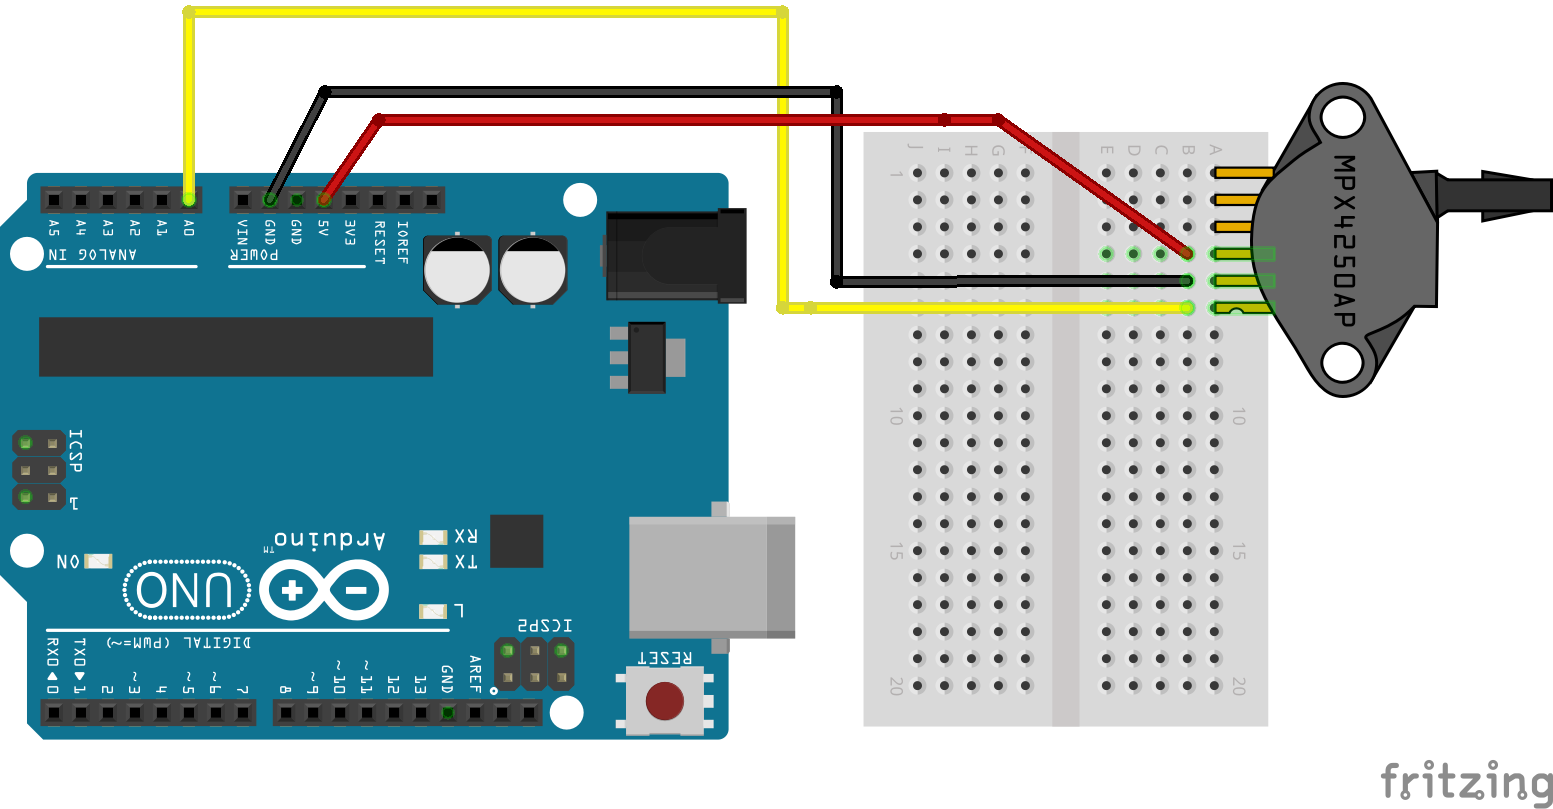
\includegraphics[scale=0.5]{images/capteurpression.png}

\end{multicols}
\textit{    les autres broches n'ont pas de fonctions sur Arduino}


\vspace{5mm}

\begin{attentionbox}
\textbf{Points de vigilance :}
\begin{itemize}
    \item Vérifiez bien les connexions avant de brancher l'Arduino
    \item Ne pas inverser l'alimentation (5V et GND)
   
\end{itemize}
\end{attentionbox}

\subsection{Questions préliminaires}

\begin{enumerate}
    \item Sur quelle broche analogique de l'Arduino est connecté le capteur ?\\
    
    \lignesreponse[1]
    
    \item Quelle est la tension maximale que peut fournir le capteur ?\\
    
    \lignesreponse[1]
    
    \item Quelle pression correspond à cette tension maximale ?\\
    
    \lignesreponse[1]
\end{enumerate}



\section{Partie 2 : Programmation de l'Arduino}

\subsection{Téléversement du programme}

Le programme \texttt{mariote.ino} est disponible sur l espace commun. Il permet de :
\begin{itemize}
    \item Lire la tension fournie par le capteur
    \item Convertir cette tension en pression (kPa)
    \item Afficher la valeur dans le moniteur série
    \item Envoyer les données vers Python
\end{itemize}


\textbf{Manipulation :}
\begin{enumerate}
    \item Ouvrir le fichier \texttt{mariotte.ino} dans Arduino IDE
    \item Sélectionner le bon port série (Outils $\rightarrow$ Port)
    \item Téléverser le programme vers la carte Arduino (bouton $\rightarrow$)
    \item Ouvrir le moniteur série (11520 bauds)
    \item Observer les valeurs de pression affichées
\end{enumerate}

\begin{infobox}
Le message « Téléversement terminé » doit s'afficher en bas de la fenêtre Arduino IDE. La LED TX/RX de l'Arduino clignote pendant le téléversement.
\end{infobox}

\subsection{Vérification du fonctionnement}

Avec le moniteur série ouvert, observer les valeurs affichées par le capteur.

\subsection{Questions}

\begin{enumerate}
    \item Le programme a-t-il été téléversé avec succès ? Quel message s'affiche ?\\
    
    \lignesreponse[1]
    
    \item Quelle est l'unité des valeurs de pression affichées dans le moniteur série ?\\
    
    \lignesreponse[1]
    
    \item Convertir la pression atmosphérique (environ 1013 hPa) en kPa :
    
    \vspace{5mm}
    Calcul : \dotfill
    
    \vspace{5mm}
    Résultat : \dotfill kPa
    
    \vspace{5mm}

    \item Pourquoi la pression affichée n'est pas égale à 1013 hPa ? \\

    \lignesreponse[1]

    
\end{enumerate}

\section{Partie 3 : Acquisition des données avec Python}

\subsection{Principe}

Le programme Python va :
\begin{itemize}
    \item Se connecter à l'Arduino
    \item Récupérer les mesures de pression
    \item Vous demander de saisir le volume correspondant
    \item Tracer le graphique $P = f(1/V)$
    \item Calculer la droite de régression
    \item Vérifier que $P \times V$ est constant
\end{itemize}

\subsection{Préparation de la mesure}

\textbf{Manipulation :}
\begin{enumerate}
    \item Connecter la seringue au capteur de pression
    \item Positionner le piston sur la graduation 40 mL et fermer le connecteur 
    \item Fermer le moniteur série de l'Arduino (très important !)
\end{enumerate}

\begin{attentionbox}
\textbf{Il est impératif de fermer le moniteur série Arduino avant d'exécuter le programme Python}, sinon le port série sera occupé et Python ne pourra pas se connecter.
\end{attentionbox}

\subsection{Lancement du programme Python}

\textbf{Manipulation :}
\begin{enumerate}
    \item Ouvrir le fichier \texttt{mariotte GUI.py} avec EduPython 
   
    \item Exécuter le programme (F5 ou bouton « Exécuter »)

\end{enumerate}

\subsection{Protocole de mesure}

Le programme va vous guider pour effectuer les mesures :

\begin{enumerate}
    \item Modifier le volume de la seringue (compression ou détente)
    \item Attendre quelques secondes que la pression se stabilise
    \item Appuyer sur \textbf{Ajouter valeur}
    \item le point s affiche dans les deux graphique
    \item Répéter l'opération pour chaque mesure
\end{enumerate}

\begin{infobox}
\textbf{Conseils pour de bonnes mesures :}
\begin{itemize}
    \item Varier le volume entre 20 mL et 60 mL environ
    \item Effectuer des mesures en compression ET en détente
    \item Bien stabiliser la pression avant de valider
    \item Noter précisément le volume sur la seringue
\end{itemize}
\end{infobox}


\section{Partie 4 : Exploitation des résultats}

\subsection{Analyse du graphique}

Le programme Python trace automatiquement le graphique représentant la pression $P$ en fonction de l'inverse du volume $\frac{1}{V}$.

Une droite de régression linéaire est calculée avec l'équation :

$$P = a \times \frac{1}{V} + b$$

où :  $a$ est le coefficient directeur et  $b$ est l'ordonnée à l'origine


\subsection{Questions d'analyse}

\vspace{5mm}

\begin{enumerate}
    \item Quelle est l'allure du graphique obtenu a droite ? \\
    
    \lignesreponse[1]
    \item Relever les valeurs affichées par le programme Python :
    
    \vspace{3mm}
    Coefficient directeur : $a = $ \dotfill kPa·mL
    
    \vspace{3mm}
    Ordonnée à l'origine : $b = $ \dotfill kPa
    
    \vspace{3mm}
    Coefficient de corrélation : $R^2 = $ \dotfill
    

    
    \item Comparer les valeurs de $a$ et $b$. Que peut-on dire de la valeur de $b$ ?\\
    
    \lignesreponse[1]

    \item Si $b \approx 0$, quelle relation existe-t-il entre $P$ et $\frac{1}{V}$ ?\\[8mm]
    
    \lignesreponse[1]

    \item En déduire la relation entre $P$ et $V$ : \dotfill \\
    
        
    \item Cette relation est-elle en accord avec la loi de Boyle-Mariotte ? Justifier.\\[8mm]
    
    \lignesreponse[1]
    
\end{enumerate}


\subsection{Vérification de la constante $P \times V$}

Ouvrir le fichier des mesures en CSV pour cela cliquer sur le bouton sauvegarder , puis ouvrir votre fichier CSV

\subsection{Questions}

\begin{enumerate}
    \item Compléter le tableau suivant avec vos 4 premières mesures :
    
    \vspace{5mm}
    
    \begin{tabular}{|c|c|c|c|}
    \hline
    \textbf{Mesure} & \textbf{P (kPa)} & \textbf{V (mL)} & \textbf{P × V (kPa·mL)} \\
    \hline
    1 & & & \\
    \hline
    2 & & & \\
    \hline
    3 & & & \\
    \hline
    4 & & & \\
    \hline
    \end{tabular}
    
    \vspace{5mm}
    
    \item Calculer la moyenne des produits $P \times V$ :
    
    \vspace{5mm}
    
    Calcul : \dotfill
    
    \vspace{5mm}
    
    Moyenne : \dotfill kPa·mL
    
    \vspace{5mm}
    
    \item Les produits $P \times V$ sont-ils constants ? Justifier en calculant l'écart-type relatif.\\
    \lignesreponse[3]
    
    \item Prenons les premières valeurs mesurées. Calculer le produit $P_1 \times V_1$ :
    
    \vspace{2mm}
    
    $P_1 = $ \dotfill kPa \hspace{1cm} $V_1 = $ \dotfill mL
    
    \vspace{2mm}
    
    $P_1 \times V_1 = $ \dotfill kPa·mL
    
    \vspace{2mm}
    
    \item Prenons maintenant les dernières valeurs. Calculer le produit $P_2 \times V_2$ :
    
    \vspace{2mm}
    
    $P_2 = $ \dotfill kPa \hspace{1cm} $V_2 = $ \dotfill mL
    
    \vspace{2mm}
    
    $P_2 \times V_2 = $ \dotfill kPa·mL
    
    \vspace{2mm}
    
    \item Les deux produits sont-ils proches ? Calculer l'écart entre les deux :
    
    \vspace{5mm}
    
    Écart : \dotfill kPa·mL
    
    \vspace{2mm}
    
    Écart relatif : \dotfill \%
    
    \vspace{5mm}
    
    \item Conclure sur la validité de la loi de Boyle-Mariotte d'après vos résultats.\\
    
    \lignesreponse[1]
\end{enumerate}
\end{document}